\documentclass{SGGW-thesis-EN}
\usepackage[utf8]{inputenc}
\usepackage{tabularx}
\usepackage{tikz}
\usepackage{listings}
\usepackage{xcolor}
\usepackage{booktabs}
\usepackage[
  backend=biber,
  style=numeric,     
  sorting=none,       
  giveninits=true,     
  maxbibnames=3,       
  doi=false,   
  isbn=false,          
]{biblatex}


\lstdefinelanguage{yaml}{
  keywords={true,false,null,yes,no},
  keywordstyle=\color{blue},
  basicstyle=\ttfamily\small,
  sensitive=false,
  comment=[l]{\#},
  morecomment=[l]{\#},
  morestring=[b]",
  morestring=[b]'
}
\usetikzlibrary{positioning, arrows.meta, shapes.geometric}
\addbibresource{references.bib}

\MASTERtrue
\WZIMtrue

\title{Development of an End-to-End OCR and NLP Pipeline for Automated Extraction and Classification of Product Data in Retail Receipts}

\Ptitle{Opracowanie systemu OCR i NLP do automatycznego wydobywania i klasyfikacji informacji o produktach z paragonów}
\author{Michał Zaręba}
\date{2025}
\album{196218}
\thesis{Diploma thesis in the field of}
\course{Information Science}
\promotor{dr hab.\ inż.\ Leszek Chmielewski, prof.\ SGGW}
\pworkplace{Institute of Information Technology\\Department of Artificial Intelligence}

\usepackage{hyperref}

\begin{document}
\maketitle
\statementpage
\abstractpage
{Pełny system ekstrakcji i klasyfikacji informacji o produktach z paragonów w języku polskim}
{Praca prezentuje end-to-end system do ekstrakcji i kategoryzacji informacji o produktach z paragonów w języku polskim. 
Modularny workflow―OCR, wstępne przetwarzanie tekstu, generowanie embeddingów i klasyfikacja―umożliwia niezależną ocenę każdego komponentu. 
Dane bazowe obejmują 26 zeskanowanych paragonów (292 wpisy), ręcznie oznaczonych w sześciu kategoriach produktowych. 
Aby zniwelować nierównowagę klas, do zbioru treningowego dodano 163 syntetycznych wpisy wygenerowanych przez GPT-4 w kontrolowanych warunkach augmentacji.
Porównano dwa podejścia do embeddingów: wstępnie wytrenowany Polish BERT (\texttt{dkleczek/bert-base-polish-cased-v1}) użyty bez dalszego fine-tuningu 
oraz mniejszy \texttt{all-MiniLM-L6-v2} (Sentence-BERT) dostrojony na danych z paragonów, z lub bez przykładów GPT.
Klasyfikator XGBoost był osobno strojon y pod każdy rodzaj embeddings, wykorzystując stały podział na zbiór walidacyjny. 
Ewaluację przeprowadzono za pomocą accuracy oraz mikroważonego i makroważonego F\textsubscript{1}.
Najlepsze rezultaty osiągnięto, gdy MiniLM dostrojono wyłącznie na prawdziwych wierszach paragonów, 
a XGBoost trenowano na mieszance oryginalnych i GPT-zbalansowanych danych. Ta konfiguracja uzyskała micro-weighted F\textsubscript{1}=0,81 i dokładność 79,6 \%. 
Fine-tuning na mieszanych danych podwyższył makroważone F\textsubscript{1} do 0,77, kosztem nieznacznego spadku accuracy.
Model Polish BERT bez fine-tuningu uzyskał gorsze wyniki (mikro-F\textsubscript{1}=0,71) i charakteryzował się wolniejszą inferencją, 
co podkreśla zalety dostosowania do domeny i stosowania lżejszych architektur.}
{OCR, NLP, BERT, Sentence-BERT, XGBoost, Generowanie danych, Nierówność Klas}
{End-to-End Extraction and Classification of Product Information from Polish Retail Receipts}
{This thesis presents an end-to-end system for extracting and categorizing product information from Polish-language receipts. 
The modular pipeline―OCR, text preprocessing, embedding generation and classification―allows each component to be developed and evaluated independently. 
The core dataset comprises 26 scanned receipts (292 line items) manually labeled into six categories. 
To address class imbalance, 163 synthetic entries generated by GPT-4 were added solely to the training pool under controlled augmentation settings.
Two embedding strategies were compared: a pretrained Polish BERT model (\texttt{dkleczek/bert-base-polish-cased-v1}) used without fine-tuning, 
and a smaller \texttt{all-MiniLM-L6-v2} Sentence-BERT model fine-tuned on receipt data (with or without GPT examples). 
An XGBoost classifier was tuned separately for each embedding source using a fixed validation split. 
Performance was measured by accuracy and micro- and macro-averaged F\textsubscript{1} scores.
The fine-tuned MiniLM encoder, trained on real receipts, combined with XGBoost on mixed real and GPT-balanced data achieved the highest 
micro-F\textsubscript{1} (0.81) and 79.6\,\% accuracy. Mixed-data fine-tuning improved macro-F\textsubscript{1} (0.77) but slightly lowered overall accuracy. 
The out-of-the-box Polish BERT underperformed (micro-F\textsubscript{1} 0.71) and showed slower inference, 
demonstrating the advantage of domain-specific adaptation and compact architectures.}
{OCR, NLP, BERT, Sentence-BERT, XGBoost, Data Augmentation, Class Imbalance}


\tableofcontents

\section*{Copyright notice}
\noindent
Unless otherwise indicated by a citation, all figures and diagrams in this thesis were created by the author and may be reused under the CC BY-NC licence.


\startchapterfromoddpage % niezależnie od długości spisu treści pierwszy rozdział zacznie się na nieparzystej stronie

\chapter{Introduction}

\section{Motivation}
Tracking expenses and managing personal finances are important aspects of modern life.
With an increasing number of daily transactions and a vast variety of products available,
individuals face significant challenges in effectively monitoring their spending and managing
their budgets.
Although receipts contain valuable details that could help consumers analyse and control their
expenses, the majority of shoppers either discard receipts shortly after purchase or find manual
analysis too tedious and time-consuming.
Automating the extraction and categorisation of product information from receipts could
significantly simplify budget tracking and provide actionable insights into spending habits,
enabling consumers to understand precisely where their money goes.
Yet, few existing tools reliably process unstructured, Polish-language receipts at the line-item level,
leaving a gap that this thesis aims to fill.
A simple and efficient way to track expenses is therefore essential for individuals who wish to
maintain a clear overview of their spending habits and make informed financial decisions.

\section{Problem Statement}
Most existing expense-tracking solutions focus on invoices, bank statements, or require manual input.
Large corporations and organisations typically possess the budgets and technical resources to deploy robust,
automated systems that extract and categorise expense data from structured documents such as invoices.
For personal use, however, the most practical source of spending information remains paper receipts.
Current receipt-based tools are often limited: many are designed exclusively for commercial purposes,
lack support for languages other than English,
or are inadequately trained to process Polish-language receipts accurately.
Thus, a clear gap exists for a solution that automatically extracts and categorises line-item product details
from receipts while accommodating the linguistic complexity of Polish.


\section{Objectives of the Study}

This study has \textbf{three concrete objectives}, each derived from the challenges set out in the problem statement:

\begin{enumerate}
  \item Extract line-item text from Polish-language receipts using Tesseract OCR combined with
        lightweight heuristic pre- and post-processing.

  \item Investigate two sentence-embedding models for representing product descriptions:
        the Polish BERT baseline, used without fine-tuning, and the \texttt{all-mini-l6-v2} model from
        the \emph{sentence-transformers} library, fine-tuned on the domain dataset.

  \item Train and evaluate an XGBoost classifier on the resulting embeddings, systematically
        comparing configurations to identify the combination that yields the highest macro-F1
        score across predefined expense categories
\end{enumerate}
\noindent
Achieving these objectives requires careful integration of OCR and NLP components as well as robust
hyper-parameter tuning to handle ambiguous, multi-word, or misspelled product names.

\section{Scope and Limitations}
The scope of this study is limited to developing a system that automatically extracts product information
from receipts and categorises these products into predefined classes.
The system specifically targets Polish-language receipts and will be evaluated chiefly on its ability to
extract item prices accurately and assign correct product categories.

\paragraph{Limitations}

\begin{itemize}
  \item The system will \emph{not} provide additional features such as longitudinal expense tracking,
        financial-report generation, or integration with external personal-finance applications.
  \item The scarcity of comprehensive, labelled Polish-language receipt datasets restricts the potential
        accuracy and generalisation capability of the developed models.
        Consequently, performance may degrade on receipt formats or lexical variants absent from the
        training data.
  \item OCR is applied without utilising spatial layout information (e.g.\ bounding boxes or reading order).
        Therefore, image preprocessing—cropping, alignment, and noise reduction—is required to supply
        clean, line-level input to the OCR engine.
\end{itemize}


\chapter{Literature Review}

\section{Optical Character Recognition (OCR) Technologies}

Optical Character Recognition (OCR) is the process of converting textual information
from scanned or photographed images into machine-readable formats.
Traditional OCR techniques relied on template matching, statistical classification and
structural analysis but offered limited adaptability to varying fonts and noisy inputs~\cite{ocrsystems}.
Modern systems employ deep-learning pipelines that combine convolutional neural networks
(CNNs) for feature extraction with recurrent or attention-based architectures—such as
LSTM or GRU layers—for sequence modelling~\cite{shi2017e2eseq}.

Recent approaches add attention mechanisms so the network can focus dynamically on
salient regions of an image.
Although LayoutLM is primarily a document-understanding model rather than an OCR engine,
it demonstrates how incorporating 2-D positional embeddings yields substantial gains on
structured documents like receipts~\cite{li2020layoutlm}.
Despite these advances, attention-based models require large, annotated datasets;
consequently the OCR tools evaluated in this study—Tesseract and PaddleOCR—operate at the
text-line level and do not encode full document layout.

\paragraph{Tesseract.}
Tesseract is a widely adopted, open-source engine maintained by Google.
It supports more than 100 languages, including Polish, and can be fine-tuned on
domain-specific data for higher accuracy.
Since version 4.0 it has featured an LSTM-based recogniser, improving robustness on
noisy or multilingual inputs~\cite{smith2007overview,smith2013history}.
Tesseract exposes numerous configuration options—segmentation modes, character
whitelists and custom language packs—allowing practitioners to tailor the engine to
narrow formats such as Polish retail receipts.

\paragraph{PaddleOCR.}
PaddleOCR is an open-source, deep-learning OCR framework developed by Baidu that currently
supports more than eighty languages~\cite{du2020ppocr}.
It offers an end-to-end, modular pipeline consisting of text detection, detected-box
rectification, and text recognition, which simplifies component-level optimisation.
Thanks to extensive data-augmentation strategies, the framework strikes a favourable
balance between accuracy and inference speed, making it suitable for real-time and
mobile scenarios.
Text detection is handled by \textit{Differentiable Binarisation}, a lightweight
segmentation network whose simplicity—augmented by minimal post-processing—maintains
high recall and precision.
The resulting bounding boxes are rectified via a text-direction classifier and then
passed to the text-recognition module.
This recogniser employs a convolutional recurrent neural network~(CRNN) architecture,
combining convolutional layers with recurrent layers to capture both local and
sequential character features.
Additional enhancements, such as a lighter backbone and task-specific augmentation,
further improve performance while preserving low-latency requirements.


\begin{figure}[h]
  \centering
  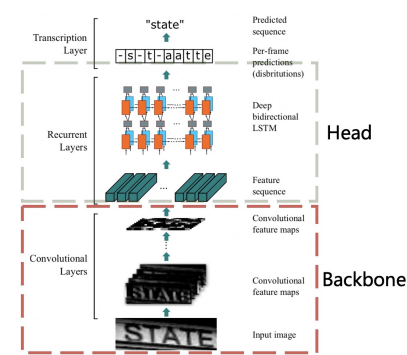
\includegraphics[width=1\textwidth]{images/cnn_text_recognizer.png}
  \caption{CRNN text recognition architecture~\cite{shi2017e2eseq}.}
  \label{fig:cnn_text_recognizer}
  \end{figure}
\begin{figure}[h]
  \centering
    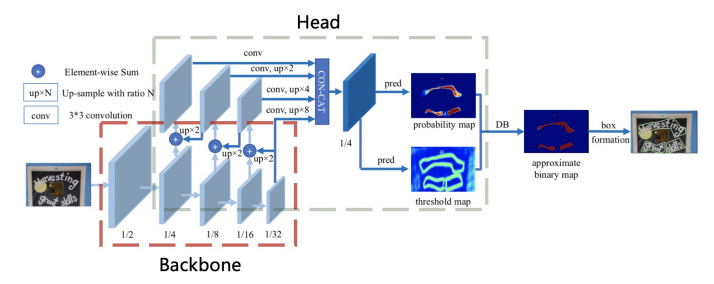
\includegraphics[width=1\textwidth]{images/text_detector_db.png}
    \caption{DBNet text detection architecture~\cite{liao2019rttextdet}.}
    \label{fig:text_detector_db}
  \end{figure}

\section{Semantic Text Embeddings for Receipt Item Categorisation}
To enable machine-learning models to analyse text, the text must first be converted into a numerical
format—a process known as \emph{vectorisation}.
Word embeddings are fixed-length vectors that encode semantic meaning and inter-word relationships;
words with similar meanings occupy nearby positions in the embedding space~\cite{almeida2023wordembeddingssurvey}.

\begin{figure}[h]
  \centering
  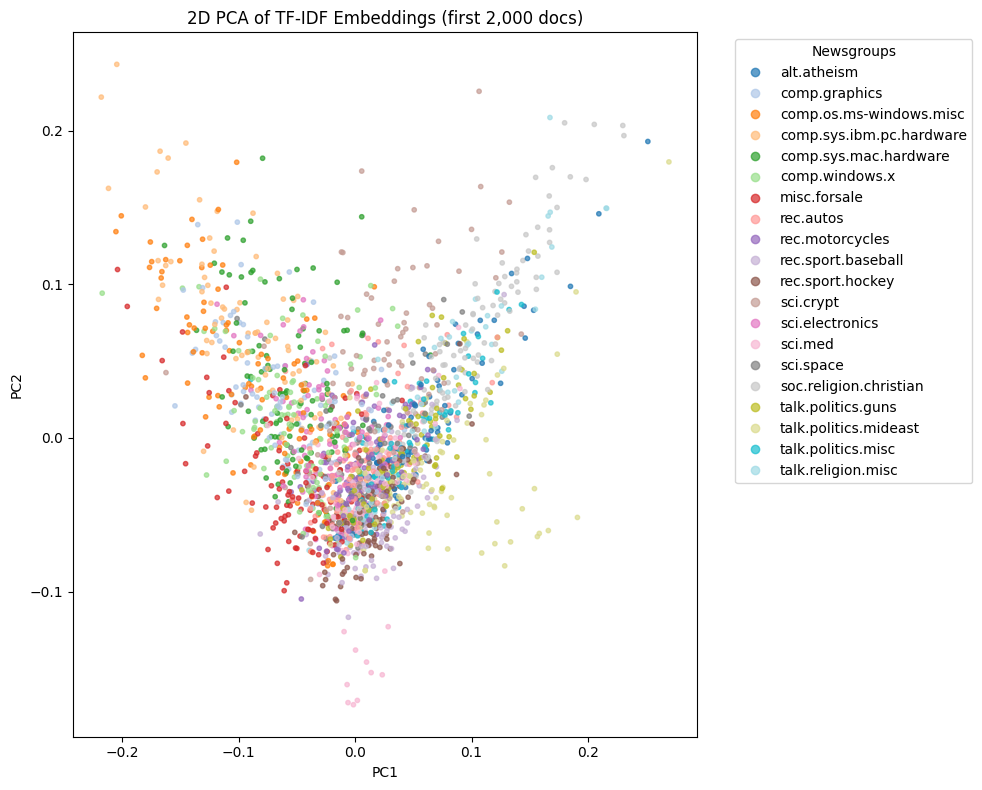
\includegraphics[height=9cm]{images/tfidf_embeddings.png}
  \caption{Two-dimensional projection of TF–IDF vectors for the \textit{20~Newsgroups} dataset (scikit-learn).}
  \label{fig:tfidf_embeddings}
\end{figure}

There are several approaches to generating embeddings.
Before embedding, the text is typically pre-processed: normalisation (e.g.\ lemmatisation or stemming)
and tokenisation, which segments text into individual words or tokens~\cite{jurafsky2023slp3}.

Embedding methods are commonly divided into two families:
\emph{count-based} techniques (e.g.\ TF–IDF, GloVe) and \emph{prediction-based} techniques (e.g.\ Word2Vec,
fastText).
The following subsections describe these groups and highlight their key differences.


\subsection{Count-based Methods}

Count-based methods rely on the premise that a word’s meaning can be inferred from how often it
co-occurs with other words in a given context.
These methods typically construct a sparse matrix whose rows and columns enumerate the
vocabulary, while each cell records the frequency of co-occurrence between word pairs.
Two common variants are the \textit{Bag-of-Words}~(BoW) model and \textit{Term Frequency–Inverse
Document Frequency}~(TF–IDF) \cite{jurafsky2023slp3}.
\paragraph{Bag-of-Words.}
BoW represents a document as an unordered vector of raw word counts, ignoring word order and
grammatical relations.

\paragraph{TF–IDF.}
TF–IDF assigns a weight to each word proportional to its frequency in the document but inversely
proportional to its frequency across the whole corpus, thereby emphasising words that are
especially informative for that document.
\subsection{Prediction-based Methods}
Prediction-based methods learn word representations by \emph{predicting} a target word from its
context—or vice versa—rather than by tallying raw co-occurrence counts.
The resulting embeddings are stored in dense matrices, which are typically more
parameter-efficient and capture semantic regularities better than the sparse matrices used by
count-based techniques~\cite{jurafsky2023slp3}.

Two widely cited prediction-based models are \textit{Word2Vec} and \textit{BERT}.
Word2Vec yields \emph{static} embeddings: each word in the vocabulary is assigned a single,
context-independent vector.
By contrast, BERT—a transformer encoder—produces \emph{contextual} embeddings whose values depend
on the surrounding tokens.

\paragraph{Word2Vec.}
Word2Vec is trained under one of two architectures:% 
\begin{enumerate}
  \item \textbf{Continuous Bag-of-Words (CBOW)} – predicts the centre (target) word from its surrounding
        context words.
  \item \textbf{Skip-Gram} – predicts surrounding context words from a single target word.
\end{enumerate}
Skip-Gram generally models rare words more faithfully, whereas CBOW offers greater computational
efficiency and shorter training times \cite{mikolov2013distributed}.

\textbf{BERT (Bidirectional Encoder Representations from Transformers)} is a deep-learning model introduced by Google that generates 
\emph{contextualised} word embeddings by processing text simultaneously in both directions (left-to-right and right-to-left).

Unlike earlier models that produce static embeddings, BERT represents each word in the context of the entire sentence, thereby capturing 
polysemy and syntactic nuance.

The underlying transformer architecture employs self-attention to weight the contribution of each token relative to all others, allowing 
the model to \emph{derive} complex semantic relationships.
BERT is pre-trained in a two-part, self-supervised scheme:
\begin{enumerate}
  \item \textbf{Masked Language Modelling (MLM)} – randomly masks a subset of input tokens and trains the network to predict the 
        masked words from their context.
  \item \textbf{Next-Sentence Prediction (NSP)} – learns to decide whether a given sentence \emph{immediately follows} another, 
        thereby improving the model’s grasp of sentence coherence.
\end{enumerate}

\begin{figure}[h]
  \centering
  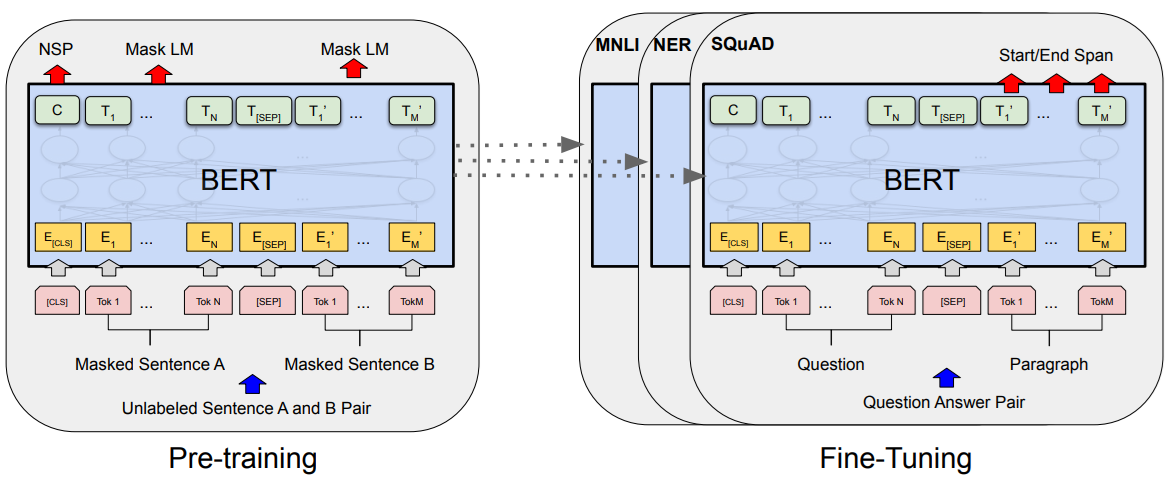
\includegraphics[height=5cm]{images/bert_procedures.png}
  \caption{Pre-training objectives of BERT: MLM and NSP \cite{devlin2019bertpretrainingdeepbidirectional}.}
  \label{fig:bert_procedures}
\end{figure}

\subsection{Sentence-BERT Embeddings}
Sentence-BERT (SBERT) adapts the original BERT into a \emph{Bi-BERT-encoder} architecture that
maps sentences to dense vectors which can be compared with simple distance measures
\cite{reimers2019sbert}.
Two weight-sharing transformer towers encode each sentence independently; a subsequent pooling
operation (typically mean pooling) yields a fixed-length embedding.
Because the sentence vectors can be pre-computed, semantic search or clustering over \(n\)
sentences requires only \(O(n)\) encoder calls, in contrast to the \(O(n^{2})\) calls needed by
cross-encoders that jointly process sentence pairs.

SBERT is trained with contrastive objectives such as \emph{natural language inference} or
\emph{triplet loss}.
During optimisation the cosine similarity between pairs of sentence embeddings is pushed high
for semantically related sentences and low for unrelated ones, thereby structuring the
embedding space for downstream tasks such as receipt-item categorisation.

\paragraph{MiniLM backbone.}
MiniLM is a distilled transformer that compresses BERT into a lighter model by matching
self-attention distributions and hidden-state relations while reducing depth and width
\cite{wang2020minilm}.
Its efficiency makes it attractive for real-time or resource-constrained deployments without
a dramatic drop in accuracy.

\paragraph{\texttt{all-mini-l6-v2}.}
The model \texttt{all-mini-l6-v2}—provided by the \emph{sentence-transformers} library is a
six-layer SBERT distilled from \texttt{microsoft/MiniLM-L12-H384-uncased} and further
fine-tuned on \(\sim 1\) billion sentence pairs~\cite{reimers2021allminilm}.
Fine-tuning employs a batch-wise contrastive objective: the cosine similarity is computed for
each possible pair of sentences within a batch, and the model is optimised so that positive
pairs obtain higher similarity scores than negative pairs.
With 384-dimensional embeddings and a footprint of roughly 90 MB,
\texttt{all-mini-l6-v2} offers an excellent speed–accuracy trade-off, which this thesis
leverages for real-time categorisation of Polish receipt items.

Contextual embeddings produced by transformer-based models have shown strong performance in a
wide range of NLP tasks, including text classification~\cite{devlin2019bertpretrainingdeepbidirectional}.

In the present study, embeddings generated by pre-trained BERT variants are used as feature
vectors for a classifier that assigns receipt items to predefined expense categories.

\section{XGBoost Classifier}

XGBoost (\emph{eXtreme Gradient Boosting}) is an open-source library that implements gradient-
boosted decision trees.
It consistently delivers state-of-the-art accuracy on a wide range of supervised-learning tasks~\cite{Chen_2016}.

Gradient boosting is an ensemble technique that, rather than fitting a single model,
\emph{builds} an initial weak learner and then iteratively fits additional learners that
minimise the residual loss~\cite{natekin2013gradient}.

\paragraph{Key design features.}
\begin{enumerate}
  \item \textbf{Regularisation} – penalises overly complex trees, thereby reducing over-fitting and
        improving generalisation.
  \item \textbf{Second-order optimisation} – uses both the gradient and the Hessian of the loss to
        approximate the objective, which accelerates convergence and improves estimation accuracy.
  \item \textbf{Shrinkage (learning rate)} – scales each tree’s contribution by a small factor after
        every boosting step, allowing the ensemble to learn gradually and robustly.
  \item \textbf{Column subsampling} – randomly selects subsets of features when growing each tree,
        further mitigating over-fitting and speeding up training.
\end{enumerate}
The final model is the sum of many shallow decision trees; each tree corrects the errors of the
ensemble built so far, and their aggregated outputs yield the prediction.

Mathematically, the ensemble prediction for an instance \(x_i\) is

\begin{figure}[h!]
  \centering
  \begin{minipage}[c]{0.40\textwidth}
    \[
      \hat{y}_i = \sum_{k=1}^{K} f_k(x_i)
    \]
  \end{minipage}\hfill
  \begin{minipage}[c]{0.55\textwidth}
    \centering
    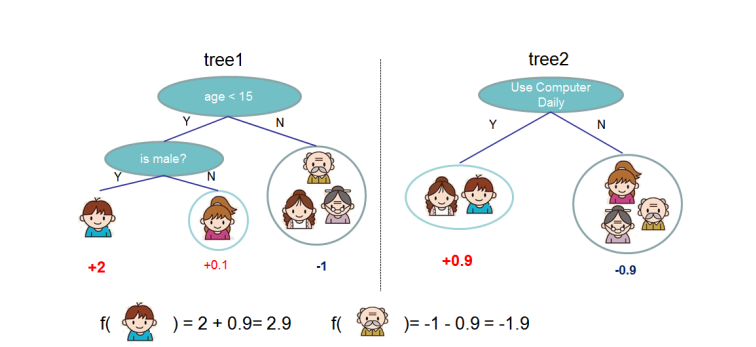
\includegraphics[width=\linewidth]{images/tree_ensemble_model.png}
    \caption{Tree-ensemble model~\cite{Chen_2016}.}\label{fig:tree_ensemble_model}
  \end{minipage}
\end{figure}
\noindent During training, XGBoost optimises a second-order Taylor expansion of the loss, which
determines the optimal structure and weights of the next tree.
The per-iteration objective simplifies to

\begin{figure}[h!]
  \centering
  \begin{minipage}[c]{0.45\textwidth}
    \[
      \tilde{\mathcal{L}}^{(t)}(q) =
      -\frac{1}{2}\sum_{j=1}^{T}
      \frac{\bigl(\sum_{i \in I_j} g_i\bigr)^2}
           {\sum_{i \in I_j} h_i + \lambda}
      \;+\; \gamma T
    \] 
  \end{minipage}\hfill
  \begin{minipage}[c]{0.55\textwidth}
    \centering
    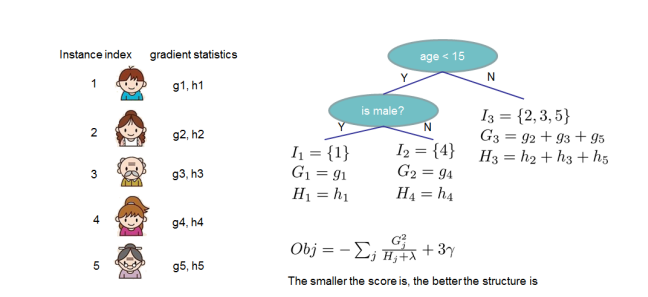
\includegraphics[width=\linewidth]{images/structure_score_calculation.png}
    \caption{Structure-score calculation~\cite{Chen_2016}.}
    \label{fig:structure_score_calculation}
  \end{minipage}
\end{figure}
\noindent where, \(g_i\) and \(h_i\) denote the first and second-order gradient statistics of the loss with
respect to the current prediction, while \(\gamma\) and \(\lambda\) are hyperparameters that penalise
complex trees and thus curb over-fitting.
In XGBoost these hyperparameters govern the trade-off between model complexity and
generalisation.

\begin{table}[h]
  \centering
  \caption{Principal XGBoost hyperparameters and their effects}\label{tab:xgboost_hyperparameters}
  \begin{tabularx}{\textwidth}{@{}lX@{}}
    \toprule
    \textbf{Hyper-parameter} & \textbf{Role and effect} \\ 
    \midrule
    \texttt{learning\_rate}    & Scales each tree’s contribution; lower values curb over-fitting but require more trees. \\ 
    \texttt{max\_depth}        & Upper bound on tree depth; deeper trees capture complex patterns yet risk over-fitting. \\ 
    \texttt{n\_estimators}     & Number of trees in the ensemble; more trees usually improve accuracy at the cost of runtime. \\ 
    \texttt{subsample}         & Fraction of training instances sampled per tree; values $<1$ add stochasticity and reduce over-fitting. \\ 
    \texttt{colsample\_bytree} & Fraction of features sampled per tree; decorrelates trees similarly to random forests. \\ 
    \texttt{min\_child\_weight} & Minimum sum of instance weights in a leaf; larger values force simpler splits. \\ 
    \texttt{gamma}             & Minimum loss reduction required to split; higher values prune trivial branches. \\ 
    \texttt{reg\_alpha}        & $L_{1}$ penalty on leaf weights; promotes sparsity by driving some weights to zero. \\ 
    \texttt{reg\_lambda}       & $L_{2}$ penalty on leaf weights; discourages extreme weights and thus over-fitting. \\ 
    \bottomrule
  \end{tabularx}
\end{table}
Tuning these settings balances close fit to the training data against the need for a simpler,
more generalisable model

\section{Challenges in OCR and NLP for Document Understanding}

The integration of OCR and NLP technologies for document understanding presents several
challenges, particularly with complex documents such as retail receipts.
These challenges include variability in receipt formats, image noise and distortion, and
language-specific characteristics.
Even state-of-the-art OCR systems struggle to maintain high accuracy on low-quality images but
basic image preprocessing like binarisation, denoising, and skew correction, can improve
input quality and thus OCR performance.

To enhance downstream understanding, some models employ \emph{2-D positional embeddings}.
These embeddings encode each token’s horizontal (\(x\)) and vertical (\(y\)) coordinates
whereas standard (1-D) positional embeddings capture only sequential order.
Incorporating spatial layout information helps the network model document structure more
accurately, which benefits tasks such as key-information extraction~\cite{subramani2021surveydeeplearningapproaches}.

A complementary strategy is \emph{text restoration}.
For example, an Action-Prediction Model predicts character-level correction actions on the
raw OCR output; applying these corrections raised NER performance from 0.59 to 0.895 F1 granting
a 76 \% relative gain in one study~\cite{gupte2021lightscameraactionframework}.
Such restoration can likewise boost text-classification accuracy.

A critical bottleneck for OCR research is the scarcity of \emph{labelled} datasets: every
document image must be paired with precise text annotations, an expensive requirement for
complex receipts~\cite{subramani2021surveydeeplearningapproaches}.
Limited data heightens the risk of over-fitting, where models perform well on the training
set yet generalise poorly to unseen inputs.
Synthetic data generation offers a promising remedy.
Tools such as \textit{Genalog} and recent LLM-based generators can create large, diverse
receipt corpora, alleviating the annotation burden and improving model robustness~\cite{gupte2021lightscameraactionframework}.


\chapter{Methodology}
\section{Introduction}

This chapter outlines the methodology used to develop and evaluate a system that
automatically extracts product information from \textit{Polish}-language receipts and
categorises those products into expense-related classes.

The workflow comprises five stages: data acquisition, preprocessing, embedding generation,
classification, and experimental evaluation.

The project is structured to support a systematic comparison of alternative embedding
strategies and to quantify their impact on classification performance, while remaining
scalable and adaptable to future enhancements.


\section{Research Design}
The primary objective of this study is to develop and rigorously evaluate an end-to-end system for extracting and
categorising product information from retail receipts.  To achieve this, I adopt a modular research design: each
component—OCR, embedding generation, and classification—may be created and tested independently, yet still plugs into a
single workflow.  This layout enables targeted assessment of individual modules and direct comparison between different
models and techniques.  Performance is examined in two experimental settings: an eight-class categorisation task trained
on the original data, and the same task trained on data augmented with GPT-4-generated lines.
These settings probe robustness under varying levels of complexity and data composition while keeping all other inputs
fixed.

The dataset is deliberately small: 26 scanned receipts yield 292 line-item entries.  I first reserve 30 \% (88 entries)
as a held-out test set.  From the remaining 70 \% (204 entries) I allocate 90 \% (184 entries) to training and 10 \%
(20 entries) to validation during fine-tuning.
Polish text introduces extra challenges.  Diacritical marks such as “ł”, “ó”, “ą”, and “ę” are common and, if
misrecognised by OCR, can hamper tokenisation and distort embeddings.  Receipts also contain many abbreviations or
truncated names—for example “kg”, “ZIEL.”, or “KAJZ.”.  I therefore apply targeted preprocessing: regular expressions
restore diacritics, expand frequent abbreviations, and remove superfluous whitespace, while robust embedding methods
help reduce noise from OCR errors and lexical fragmentation.

Model performance is evaluated with the micro-averaged F\textsubscript{1} score, which balances precision and recall
over all classes.  As a baseline for tokenisation and embedding, I use the Polish BERT model
\texttt{dkleczko/bert-base-polish-uncased-v1}~\cite{kleczek2020polbert},
whose sub-word vocabulary is well suited to Polish diacritics and inflection.  The OCR stage remains PaddleOCR in every
experiment. Comparing this BERT baseline with stronger embedding models and an XGBoost classifier quantifies the gains delivered by more advanced
representations.

\begin{figure}[h]
  \centering
  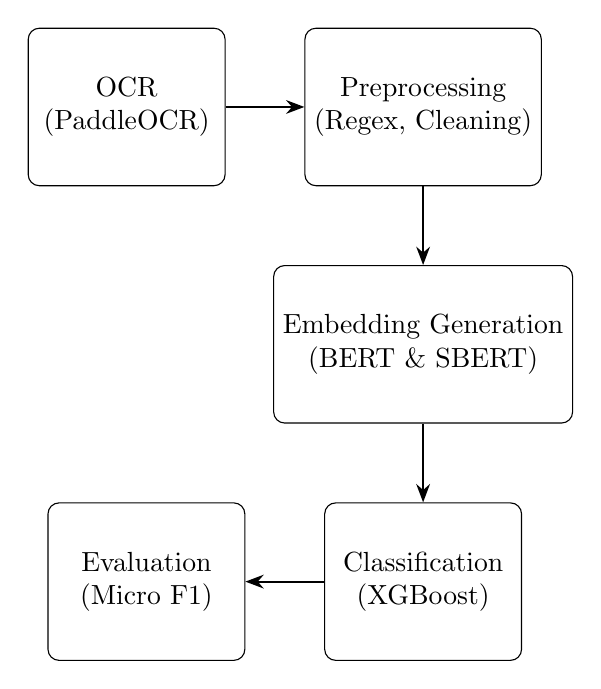
\begin{tikzpicture}[
      box/.style={
        rectangle,
        draw,
        rounded corners,
        minimum width=2.5cm,
        minimum height=2cm,
        align=center
      },
      >={Stealth},
      every edge/.style={draw, thick, -{Stealth}},
      node distance=1cm
    ]
    \node[box] (ocr) {OCR\\(PaddleOCR)};
    \node[box, right=of ocr] (pre) {Preprocessing\\(Regex, Cleaning)};
    \node[box, below=of pre] (emb) {Embedding Generation\\(BERT \& SBERT)};
    \node[box, below=of emb] (clf) {Classification\\(XGBoost)};
    \node[box, left=of clf] (eval) {Evaluation\\(Micro F1)};

    \path (ocr) edge (pre)
          (pre) edge (emb)
          (emb) edge (clf)
          (clf) edge (eval);
  \end{tikzpicture}
  \caption{High-level flowchart of the receipt-processing and classification pipeline.}
  \label{fig:pipeline_flowchart_vertical}
\end{figure}



\section{Data Sources, Collection and Preparation}

\subsection{Data Acquisition and Annotation}
The dataset comprises 292 line-item entries extracted from 26 scanned receipts using PaddleOCR.
To address class imbalance, 163 synthetic entries were generated with GPT-4, focusing on the least-represented categories. 
Each record was manually annotated with one of six product classes (Food, Beverages, Housing, Healthcare, Discount, Other) together
with the corresponding cost.

\subsection{Data Pipeline and Loading}
My pipeline begins by reading an annotated \texttt{CSV} file with three columns:
\begin{itemize}
  \item \textbf{Text}: the receipt line item recognised by OCR,
  \item \textbf{Category}: the manual label (six classes), 
  \item \textbf{Cost}: the monetary value of the item.
\end{itemize}
A label encoder converts the categorical labels into numeric codes. Prior to embedding and classification, each text
line is normalised to reduce noise: punctuation is replaced with spaces to separate tokens, consecutive spaces are
collapsed to one, citation-like patterns produced by OCR are removed, non-alphanumeric characters (except whitespace)
are stripped, digits are dropped to avoid price leakage, and single-letter tokens are discarded because they rarely
carry meaning in this domain.

These preprocessing operations standardise the textual data and ensure that only informative content reaches the
embedding models and classifier.  The original dataset (292 entries) is first divided with stratified sampling: 70 \%
(204 entries) forms the training pool and 30 \% (88 entries) forms the fixed test set.  The training pool is then split
again so that 90 \% (184 entries) is used for model fitting and 10 \% (20 entries) for validation.  Synthetic GPT-4
examples are added \emph{only} to the training portion (184 entries) when the augmentation setting is evaluated, while
validation and test sets remain unchanged; this guarantees that test metrics are computed solely on real receipt data.


\subsection{Class Distribution Analysis}
Figure~\ref{fig:dist_6class} compares two datasets employed in this study: 
the original OCR‐extracted receipt data, and a supplementary dataset generated with GPT. The latter was designed for equal class
representation and is therefore referred to as the “balanced” GPT dataset.

Within the six‐class taxonomy, the original receipt data exhibit pronounced imbalance. The \emph{Food} category
dominates, accounting for more than half of all items, whereas other categories—such as \emph{Beverage}
and \emph{Healthcare}—contain only a handful of examples.  Such skew is expected because food purchases are typically the
most frequent; however, it complicates classification, as models trained on imbalanced data tend to favour majority
classes.  By contrast, the GPT‐generated dataset provides roughly equal sample counts per class.  Although this balance
introduces diversity and bolsters minority categories, the resulting distribution does not mirror real‐world receipts.
Balancing categories is valuable during augmentation, yet synthetic data used for training should align with empirical
class frequencies.  A marked mismatch between the GPT and original datasets risks overfitting to artificial proportions
rather than learning meaningful distinctions.  Accordingly, GPT‐generated samples ought to be resampled to reflect the
observed class distribution before training.
Maintaining comparable distributions across all subsets ensures that the classifier encounters realistic category
ratios, and that performance comparisons reflect genuine model capability rather than artefacts stemming from skewed or
overly uniform training inputs.

\begin{figure}[h]
  \centering
  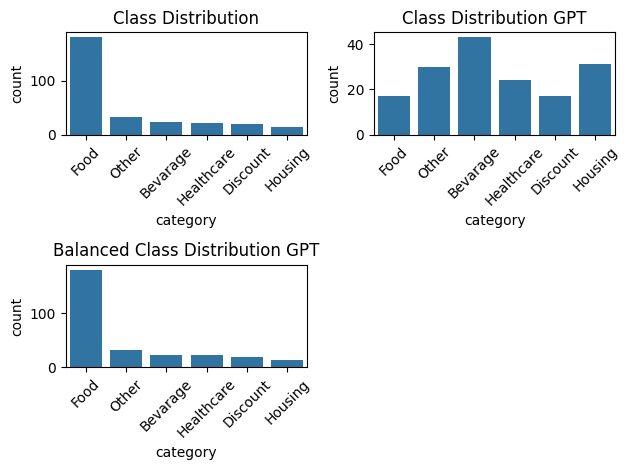
\includegraphics[width=0.8\textwidth]{images/class_distribution.png}
  \caption{Original, GPT-augmented, and balanced class distributions.}
  \label{fig:dist_6class}
\end{figure}

\subsection{Embedding Generation}
Two embedding approaches are evaluated and compared.  The first employs the pre-trained Polish BERT model
\texttt{dkleczko/bert-base-polish-uncased-v1}, which produces token-level contextual representations based on a broad
Polish corpus.  As this model is not fine-tuned for receipt classification, it functions as a strong, general-purpose
baseline.

The second approach relies on the \texttt{all-MiniLM-L6-v2} Sentence-BERT model—a lighter, sentence-level encoder that
has been fine-tuned on receipt-related data to capture domain-specific semantics relevant to product categorisation.

The two models are applied in separate pipelines rather than combined; their performances are compared to examine how
domain adaptation and model size influence results.  In each case, the generated embeddings serve as input features for
the XGBoost classifier.



\section{Modelling and Analysis}
This section describes the experiment design and the rationale for the chosen comparisons. Each receipt line is first
converted into a fixed-length vector, then classified with XGBoost. The vector is produced by one of two embedding
models, evaluated separately.

\textbf{Embedding sources.} The general-purpose baseline is the Polish BERT model
\texttt{dkleczek/bert-base-polish-uncased-v1}, pretrained on a broad Polish corpus and left unchanged for this task. The
second source is \texttt{all-MiniLM-L6-v2}, a lighter Sentence-BERT model fine-tuned on receipt data to capture
domain-specific meaning. The two models are assessed in parallel and never combined.

\textbf{Hyper-parameter search.} XGBoost settings—learning rate, tree depth, number of estimators and regularisation—are
optimised with a simple search that uses a fixed validation set drawn once from the training pool. No cross-validation
is applied, and the same train–validation split (defined with a fixed random seed) is reused in every trial.

\textbf{Taxonomy and metrics.} Classification follows an six-class scheme. Training, validation and test splits remain
identical across embedding types, ensuring fair comparison. Performance is reported with the macro-averaged
F\textsubscript{1} score, which gives equal weight to every class and therefore counteracts the natural imbalance found
in real receipts.

This setup isolates the impact of embedding choice and tailored hyper-parameter tuning while keeping all other factors
constant.

\section{Experimental Setup and Evaluation}
Hydra manages all experiment configurations, ensuring exact reproduction of every run. The held-out test set is fixed
and contains only real receipt lines; it is never exposed during training or validation.

\subsection*{Embedding variants}
\begin{enumerate}
  \item \textbf{Polish BERT baseline} (\texttt{dkleczek/bert-base-polish-uncased-v1})\,: pretrained, no task-specific
        fine-tuning.
  \item \textbf{MiniLM–receipts}\,: \texttt{all-MiniLM-L6-v2} fine-tuned on the original receipt corpus.
  \item \textbf{MiniLM–receipts+GPT}\,: the same MiniLM model further fine-tuned with GPT-generated lines.
\end{enumerate}

\subsection*{Dataset variants}
Two orthogonal switches control the training data:
\begin{itemize}
  \item \textbf{Augmentation}\,: GPT lines either included (\emph{augmented}) or excluded (\emph{non-augmented}).
  \item \textbf{Balancing}\,: when GPT lines are used, they are kept uniform (\emph{balanced}) or resampled to mirror the
        empirical class frequencies (\emph{not-balanced}).
\end{itemize}

Combining the three embeddings with these dataset options yields twelve distinct scenarios. Hyper-parameters for
XGBoost—learning rate, tree depth, number of estimators and regularisation—are optimised separately for every scenario
using a fixed train–validation split created once with a deterministic seed.

Accuracy and macro-averaged F\textsubscript{1} scores for most important runs are presented in Chapter~V.

\section{Summary}
The methodology outlined in this chapter links OCR text extraction, manual annotation, targeted preprocessing and
embedding features with an XGBoost classifier. The experimental framework supports systematic comparison across three
embedding variants—Polish BERT, MiniLM fine-tuned on receipts and MiniLM fine-tuned with both receipts and GPT
examples—and tests each model under several training conditions that vary augmentation and balancing. This design
provides a reliable basis for judging how embedding choice, data composition and tailored hyper-parameter search affect
multi-class product categorisation performance on receipt data.


\chapter{Implementation}

\section{Overview}
The implemented system follows a modular pipeline with separate components for data loading, preprocessing,
embedding generation, model training and evaluation. Each component is developed independently and connected through
centralised configuration files managed by Hydra.

This design permits straightforward substitution of embedding methods, classification algorithms and data sources
without extensive code changes. All settings—hyper-parameters, dataset versions and experiment definitions—are recorded
in Hydra, which guarantees consistent and reproducible runs.

Written entirely in Python, the code prioritises readability, extensibility and repeatability. The framework supports
multiple embedding models and can switch seamlessly between pretrained and fine-tuned variants. Results, logs and
artifacts are stored in a structured directory tree, making later comparison and analysis easier.


\section{Technology Stack}
The system relies on a set of well-established tools chosen for robustness, efficiency and ease of extension:

\begin{itemize}
  \item \textbf{Programming language} – Python 3.12, selected for its rich ecosystem and mature support for machine-learning,
        NLP and computer-vision tasks.
  \item \textbf{OCR} – PaddleOCR, valued for its modular design, multilingual coverage and reliable recognition of Polish text.
  \item \textbf{Embedding models}
        \begin{itemize}
          \item \texttt{dkleczek/bert-base-polish-uncased-v1} for general-purpose Polish \newline contextual embeddings.
          \item \texttt{all-MiniLM-L6-v2} fine-tuned on receipt data for domain-specific semantics.
        \end{itemize}
  \item \textbf{Classifier} – XGBoost, chosen for speed, scalability and strong performance.
  \item \textbf{Supporting libraries}
        \begin{itemize}
          \item \texttt{Transformers} for loading and managing pre-trained language models.
          \item \texttt{SentenceTransformers} for fine-tuning and embedding generation.
          \item \texttt{scikit-learn} for preprocessing utilities and evaluation metrics.
        \end{itemize}
  \item \textbf{Configuration} – Hydra, providing centralised, reproducible experiment management.
  \item \textbf{Visualisation} – Matplotlib (and optional Seaborn) for exploratory plots and metric charts.
  \item \textbf{System dependencies}
        \begin{itemize}
          \item \texttt{CUDA} and \texttt{PyTorch} for GPU-accelerated training and inference.
          \item \texttt{OpenCV} for image preprocessing tasks such as resizing, binarisation and noise reduction.
        \end{itemize}
\end{itemize}

This stack balances performance, seamless integration and future extensibility, ensuring reliable and reproducible
experiments.

\section{System Architecture}
The system follows a modular design organised into five sequential components, each responsible for a distinct step in
the processing pipeline:

\begin{itemize}
  \item \textbf{OCR module} – extracts text from scanned receipt images with PaddleOCR.
  \item \textbf{Pre-processing module} – cleans and normalises the text, handling Polish diacritics, abbreviations and
        common OCR errors.
  \item \textbf{Embedding module} – converts normalised text into numerical vectors using either Polish BERT or the
        fine-tuned Sentence-BERT model.
  \item \textbf{Classification module} – assigns each line item to a predefined expense class with XGBoost.
  \item \textbf{Evaluation module} – reports accuracy and macro-averaged F\textsubscript{1} scores.
\end{itemize}

This structure allows any component to be developed, replaced or extended without affecting the others, making it
straightforward to test new models or processing techniques. The data flow between modules is illustrated in
Figure~\ref{fig:pipeline_flowchart_vertical} in the “Research Design” section.

\section{Component Implementation}

\subsection{DataLoader and Input Handling}
The \textit{DataLoader} module ingests CSV files that contain receipt line-item text, annotated product categories and
associated costs. It processes two data sources in a unified way: (i) the original OCR-extracted receipts and (ii)
synthetic lines generated with GPT.

To reduce class imbalance in the training data, the module applies random undersampling by drawing examples from each
category until all classes reach the same frequency. The balanced subset is then passed to later stages, helping the
classifier avoid bias towards majority categories.


\subsection{Pre-processing Module}
The pre-processing module cleans and standardises the raw text produced by OCR. Regular expressions remove punctuation,
numerical artefacts and citation-like patterns, after which all characters are converted to lower case and consecutive
whitespace is collapsed. Polish-specific steps then restore diacritics and expand common abbreviations commonly seen in
receipts. These transformations yield uniformly formatted text that is well suited to the downstream embedding and
classification stages.


\subsection{Embedding Interface}
The \textit{Embedding} module offers a uniform method for converting pre-processed text into numerical
vectors. Two transformer-based strategies are supported:

\begin{itemize}
  \item \textbf{Polish BERT} (\texttt{dkleczek/bert-base-polish-uncased-v1})\,: generates token-level contextual embeddings
        that reflect general Polish semantics and syntax.
  \item \textbf{Sentence-BERT} (\texttt{all-MiniLM-L6-v2})\,: produces sentence-level embeddings and is fine-tuned on
        receipt data to capture domain-specific nuances.
\end{itemize}

The interface handles model initialisation, tokenizer setup, batch processing and the extraction or aggregation of
embedding vectors. This standardised workflow ensures compatibility with downstream tasks such as classification.


\subsection{Training and Evaluation Pipeline}
The training pipeline applies XGBoost for supervised categorisation of receipt line items. Its main duties are:
\begin{itemize}
  \item fitting the classifier on numerical embeddings with the annotated product classes as targets;
  \item dividing the data—once, with a fixed random seed—into training and validation subsets for hyper-parameter
        tuning;
  \item recording all settings in Hydra configuration files so that hyper-parameters, data paths and model options are
        exactly reproduced in every run.
\end{itemize}

The evaluation stage reports accuracy and the macro-averaged F\textsubscript{1} score, providing a consistent basis for
comparing different embedding methods and experiment configurations.


\section{Training Configuration}
The experiments were run on the hardware and software stack listed below. All values are reported to aid reproducibility
and allow direct comparison with future work.

\begin{itemize}
  \item \textbf{Hardware}
        \begin{itemize}
          \item CPU: AMD Ryzen 7600
          \item GPU: NVIDIA Titan RTX
          \item RAM: 32 GB
        \end{itemize}

  \item \textbf{Software}
        \begin{itemize}
          \item Operating system: Ubuntu 22.04
          \item Python: 3.10
          \item CUDA: 11.8
          \item PyTorch: 2.0
        \end{itemize}

  \item \textbf{Reproducibility}
        \begin{itemize}
          \item Random seed: 42, fixed across all runs
          \item Logging: Hydra stores every configuration, metric and log in a structured output directory
        \end{itemize}

  \item \textbf{Approximate training time}
        \begin{itemize}
          \item XGBoost classifier: a few seconds per run
          \item Embedding fine-tuning: 5–20 min, depending on dataset size and model complexity
        \end{itemize}

  \item \textbf{Hyper-parameter search (Optuna)}
        \begin{itemize}
          \item Sentence-BERT: 1000 trials, around 1–2 h
          \item Polish BERT: 100 trials, around 1 h
        \end{itemize}
\end{itemize}
\section{Reproducibility and Setup}

To ensure reproducibility and ease of setup, the project follows a structured organization and provides clear installation instructions.

\subsection{Project Structure}
The repository is arranged as follows:
\begin{itemize}
  \item \textbf{src/}\,: main Python package
    \begin{itemize}
      \item \textbf{analysis/}\,: Jupyter notebooks for exploratory work  
            (\texttt{data\_analysis.ipynb}, \texttt{thesis\_visualisation.ipynb}, \texttt{tokenisation.ipynb})
      \item \textbf{conf/}\,: Hydra configuration
        \begin{itemize}
          \item \texttt{config.yaml}
          \item \texttt{params/}\,: additional YAML fragments
        \end{itemize}
      \item \textbf{data/}\,: organised datasets and annotations
        \begin{itemize}
          \item \texttt{annotations/}
          \item \texttt{images/}
        \end{itemize}
      \item \textbf{model/}\,: model code and artefacts
        \begin{itemize}
          \item \texttt{dataloader.py}, \texttt{classifier.py}, \texttt{embeddings.py}, \texttt{ocr.py}
          \item \texttt{xgboost\_model.json}
        \end{itemize}
      \item \textbf{scripts/}\,: stand-alone utilities (e.g.\ \texttt{annotation\_pipeline.py})
      \item \textbf{utils/}\,: shared helper functions (\texttt{utils.py})
    \end{itemize}

  \item \textbf{main.py}, \textbf{train\_model.py}\,: entry points for running the pipeline and training the model
  \item \textbf{pyproject.toml}, \textbf{uv.lock}\,: project metadata and locked dependencies
  \item \textbf{README.md}, \textbf{.gitignore}\,: documentation and Git ignore rules
\end{itemize}

\subsection{Installation Instructions}
The following steps set up the environment and reproduce the experiments:

\begin{enumerate}
  \item \textbf{Install UV} (Ultrafast Virtualenv) if it is not already present:
        \begin{lstlisting}[language=bash]
curl -LsSf https://astral.sh/uv/install.sh | sh
        \end{lstlisting}

  \item \textbf{Install project dependencies}:
        \begin{lstlisting}[language=bash]
cd /path/to/project
uv sync
        \end{lstlisting}
        This command reads the committed \texttt{uv.lock} (or \texttt{pyproject.toml}) and creates a
        \texttt{.venv/} directory automatically.

  \item \textbf{Confirm that CUDA is available for GPU acceleration}:
        \begin{lstlisting}[language=bash]
nvcc --version
        \end{lstlisting}
        Ensure that the reported CUDA version matches the one supported by the installed PyTorch build.

  \item \textbf{Run an mutirun experiment using Hydra}:
        \begin{lstlisting}[language=bash]
uv run python src/train_model.py --multirun
        \end{lstlisting}
        The command \texttt{uv run} synchronises the environment before executing the script.
\end{enumerate}

Following these steps reproduces the experiments on systems with comparable hardware and software.

\subsection{Configuration Management with Hydra}
All experiment settings are maintained in Hydra configuration files to keep code and parameters separate. This arrangement
allows rapid changes to model type, data source, embedding strategy or training hyper-parameters without touching the core
implementation.

Each run is launched with a dedicated settings that can be set up in YAML file, for example:
\begin{lstlisting}[language=yaml, caption=Sample Hydra configuration]
params:
  learning_rate: 0.3
  max_depth: 5
  n_estimators: 500
  subsample: 1.0
  colsample_bytree: 0.5
  min_child_weight: 5
  gamma: 0.1
  reg_alpha: 1.0
  reg_lambda: 1.0

embeddingmodel:
  model_path: "../finetuned_base_model"
gptdatapath: "../annotations_gpt.csv"
datapath: "../annotations_6classes.csv"
balance_data: true
split_size: 0.3
\end{lstlisting}

For every run Hydra creates a separate output directory that contains:
\begin{itemize}
  \item the exact configuration file used;
  \item all logs produced during training and evaluation;
  \item the resulting metrics.
\end{itemize}

This structure guarantees full reproducibility and makes it easy to track performance across multiple model
configurations.

\section{Summary}
The system follows a modular design with distinct components for OCR, pre-processing, embedding generation, classification
and evaluation. This structure allows flexible experimentation and straightforward integration of alternative models or
methods. Configuration management through Hydra preserves reproducibility, streamlines hyper-parameter tuning and
supports well-structured comparisons across experimental setups.


\chapter{Evaluation and Results}
\section{Experimental Setup}
Model performance was optimised with Optuna using \textbf{1 000 trials}. The TPE sampler (seed = 42) explored a wide
hyper-parameter space, aiming to maximise the micro-averaged F\textsubscript{1} score on the held-out validation split.
The search covered key XGBoost settings and categorical flags that switch embedding models and data options:

\begin{itemize}
  \item \textbf{learning\_rate}: \{0.01, 0.05, 0.1, 0.2, 0.3\}
  \item \textbf{max\_depth}: \{3, 5, 7, 10, 15, 20\}
  \item \textbf{n\_estimators}: \{50, 100, 200, 300, 500, 750, 1 000\}
  \item \textbf{subsample}: \{0.5, 0.6, 0.7, 0.8, 0.9, 1.0\}
  \item \textbf{colsample\_bytree}: \{0.5, 0.6, 0.7, 0.8, 0.9, 1.0\}
  \item \textbf{min\_child\_weight}: \{1, 2, 3, 5, 7, 10\}
  \item \textbf{gamma}: \{0.0, 0.1, 0.5, 1.0, 2.0, 5.0\}
  \item \textbf{reg\_alpha}: \{0.0, 0.1, 0.5, 1.0, 2.0, 5.0\}
  \item \textbf{reg\_lambda}: \{0.0, 0.1, 0.5, 1.0, 2.0, 5.0\}
  \item \textbf{embeddingmodel.model\_path}:\newline
  \{\textit{mini\_finetuned\_base}, \textit{mini\_finetuned\_augmented}, \textit{bert}\}
  \item \textbf{augment\_classifier}: \{True, False\}
  \item \textbf{balance\_data}: \{True, False\}
\end{itemize}

This configuration allowed Optuna to examine a broad range of model and data combinations efficiently. Although the
TPEsampler can fall into local optima, systematic exploration led to a notable improvement in classification
performance over untuned baselines.


\section{Evaluation Metrics}
Model performance is reported with four standard measures: accuracy, precision, recall and the
F\textsubscript{1}\, score. Accuracy shows the proportion of correct predictions across all classes, but it can be
misleading when data are imbalanced. Precision measures the fraction of positive predictions that are correct, whereas
recall captures the fraction of actual positives retrieved by the model.

The principal metric in this study is the \emph{micro-averaged} F\textsubscript{1} score. It pools true positives,
false positives and false negatives over all classes and is therefore well suited to imbalanced data, providing a
single figure that reflects overall effectiveness.

Alongside this, the \emph{macro-averaged} F\textsubscript{1} score is also reported. It computes an
F\textsubscript{1} value for each class and then averages them, giving equal weight to both frequent and rare
categories. Reporting both micro and macro scores offers a balanced view: the former summarises global performance,
while the latter reveals how well the classifier handles minority classes.


\section{Result Analysis}
\subsection{Best-performing model}
The strongest results were obtained with the \texttt{all-MiniLM-L6-v2} Sentence-BERT encoder, fine-tuned solely on real
receipt lines.
Classification was carried out by XGBoost trained on a mix of real and GPT-augmented data, the latter resampled to
equalise class counts. This setting reached 79.55 \% accuracy, a micro-averaged F\textsubscript{1} of 0.8053 and a
macro F\textsubscript{1} of 0.70, indicating robust performance across both frequent and rare classes.

\subsubsection*{Model configuration}
\begin{itemize}
  \item \texttt{learning\_rate}: 0.01 \quad \texttt{max\_depth}: 5 \quad \texttt{n\_estimators}: 1 000
  \item \texttt{subsample}: 1.0 \quad \texttt{colsample\_bytree}: 0.7
  \item \texttt{min\_child\_weight}: 2 \quad \texttt{gamma}: 2.0
  \item \texttt{reg\_alpha}: 0.0 \quad \texttt{reg\_lambda}: 5.0
\end{itemize}

\subsubsection*{Overall performance}
Table~\ref{tab:best_model_summary} summarises the aggregate metrics. The combination of domain-specific fine-tuning and
GPT-balanced training data delivers the most even performance among all configurations.

\begin{table}[h]
  \centering
  \caption{Overall performance—\texttt{all-MiniLM-L6-v2} fine-tuned on real data, XGBoost trained on real\,+\,GPT-balanced data}
  \label{tab:best_model_summary}
  \begin{tabularx}{\textwidth}{lccc}
    \toprule
    \textbf{Metric} & \textbf{Macro Avg} & \textbf{Weighted Avg} & \textbf{Overall Accuracy} \\
    \midrule
    Precision        & 0.74 & 0.83 & 0.7955 \\
    Recall           & 0.70 & 0.80 & 0.7955 \\
    F1 Score (Macro) & 0.70 & 0.81 & 0.7955 \\
    F1 Score (Micro) & \multicolumn{3}{c}{0.8053} \\
    Overall Accuracy & \multicolumn{3}{c}{0.7955} \\
    \bottomrule
  \end{tabularx}
\end{table}

\subsubsection*{Class-level performance}
Table~\ref{tab:best_model_report} lists per-class metrics.
High F\textsubscript{1} scores for \emph{Food} (0.88), \emph{Discount} (0.91) and \emph{Beverage} (0.83) reflect either
ample support or distinctive lexical patterns, whereas \emph{Housing} and \emph{Healthcare} remain challenging.

\begin{table}[h]
  \centering
  \caption{Detailed classification report—best model}
  \label{tab:best_model_report}
  \begin{tabularx}{\textwidth}{lcccc}
    \toprule
    \textbf{Class} & \textbf{Precision} & \textbf{Recall} & \textbf{F1 Score} & \textbf{Support} \\
    \midrule
    Beverages (0)  & 1.00 & 0.71 & 0.83 & 7  \\
    Discount  (1)  & 1.00 & 0.83 & 0.91 & 6  \\
    Food      (2)  & 0.89 & 0.87 & 0.88 & 55 \\
    Healthcare (3) & 0.36 & 0.67 & 0.47 & 6  \\
    Housing    (4) & 0.50 & 0.50 & 0.50 & 4  \\
    Other      (5) & 0.67 & 0.60 & 0.63 & 10 \\
    \midrule
    \textbf{Macro Avg}        & 0.74 & 0.70 & 0.70 & 88 \\
    \textbf{Weighted Avg}     & 0.83 & 0.80 & 0.81 & 88 \\
    \textbf{Overall Accuracy} & \multicolumn{4}{c}{0.7955} \\
    \textbf{Micro Avg F1}     & \multicolumn{4}{c}{0.8053} \\
    \bottomrule
  \end{tabularx}
\end{table}

\noindent
These results suggest that domain-specific fine-tuning preserves receipt semantics, while GPT-balanced data corrects
for class imbalance, together setting a solid benchmark for future work on receipt-based product categorisation.

\subsection{Sentence-BERT Fine-tuned on Mixed Data}
The \texttt{all-MiniLM-L6-v2} encoder was fine-tuned on a mixture of real and GPT-augmented receipt lines, whereas the
XGBoost classifier used embeddings from this encoder but was trained solely on real data. This set-up reached
78.41 \% accuracy, a weighted F\textsubscript{1} of 0.80 and a macro F\textsubscript{1} of 0.77. The overall
(micro-averaged) F\textsubscript{1} score was 0.7967, slightly below the best model, yet the higher macro figure
indicates more even class-wise performance—chiefly an improvement for the \emph{Healthcare} category.

\begin{table}[h]
  \centering
  \caption{Classification report—MiniLM fine-tuned on mixed data, XGBoost trained on real data}
  \label{tab:finetuned_st_real_clf_report}
  \begin{tabularx}{\textwidth}{lcccc}
    \toprule
    \textbf{Class} & \textbf{Precision} & \textbf{Recall} & \textbf{F1 Score} & \textbf{Support} \\
    \midrule
    Beverages (0)  & 0.88 & 1.00 & 0.93 & 7  \\
    Discount  (1)  & 1.00 & 0.83 & 0.91 & 6  \\
    Food      (2)  & 0.88 & 0.78 & 0.83 & 55 \\
    Healthcare (3) & 1.00 & 0.83 & 0.91 & 6  \\
    Housing    (4) & 0.50 & 0.50 & 0.50 & 4  \\
    Other      (5) & 0.41 & 0.70 & 0.52 & 10 \\
    \midrule
    \textbf{Macro Avg}        & 0.78 & 0.77 & 0.77 & 88 \\
    \textbf{Overall Accuracy} & \multicolumn{4}{c}{0.7841} \\
    \textbf{Micro Avg F1}     & \multicolumn{4}{c}{0.7967} \\
    \bottomrule
  \end{tabularx}
\end{table}
\noindent Although the macro-averaged scores suggest better balance, the encoder’s dependence on GPT-generated patterns differs
from the behaviour seen in the best-performing model. This discrepancy raises the possibility that the fine-tuned
Sentence-BERT has adapted too closely to synthetic text, limiting generalisability to genuine receipts. Further work
could explore regularisation or domain-adversarial training to reduce sensitivity to synthetic artefacts.


\subsection{BERT-Based Model (Out-of-the-Box)}
This experiment evaluates the pretrained Polish BERT model without any task-specific fine-tuning. Despite its larger size, it delivers lower performance across key metrics and exhibits slower inference, making it
less practical here.

The model achieved an accuracy of 72.73\,\% and a weighted F\textsubscript{1} score of 0.7073. However, the
macro-averaged F\textsubscript{1} dropped to 0.51, substantially below other configurations. This decline indicates poor
generalisation across classes, especially those with limited support or greater semantic variability.
For instance, the \emph{Food} class still shows strong recall (0.89) and F\textsubscript{1} (0.83), but other categories
perform poorly. The \emph{Beverage} class attains only 0.18 F\textsubscript{1}, and \emph{Housing} receives no correct
predictions. Such disparities confirm that the model favours majority classes and struggles with underrepresented labels.

Moreover, BERT’s large architecture increases inference time without improving accuracy. In contrast, the smaller
\texttt{all-MiniLM-L6-v2} model—fine-tuned on receipt data—yields higher scores and much faster predictions,
demonstrating its suitability for real-world applications.
A detailed classification report for this BERT configuration is provided in Appendix~\ref{appendix:bert-report-outofbox}.

\chapter{Discussion}

\section{Interpretation of Results}
Table~\ref{tab:results_comparison} compares the three model configurations evaluated in this study. The strongest
pipeline uses \texttt{all-MiniLM-L6-v2}, fine-tuned on real receipt lines, and an XGBoost classifier trained on a
combination of real and GPT-augmented samples. This configuration achieves a micro-averaged F\textsubscript{1} of 0.81
and 80\,\% accuracy. GPT augmentation appears to improve recall for under-represented classes.

Fine-tuning MiniLM on mixed real and GPT data, with XGBoost trained on real lines only, yields a slightly lower
micro-averaged F\textsubscript{1} of 0.80 but a higher macro-averaged F\textsubscript{1} of 0.77. The improved macro
score indicates more balanced performance across all categories, especially a marked gain for \emph{Healthcare}.

The pretrained Polish BERT (\texttt{dkleczek/bert-base-polish-uncased-v1}) used out of the box with XGBoost on real
data produces 0.71 micro-averaged F\textsubscript{1} and a macro-averaged F\textsubscript{1} of 0.51, reflecting poor
generalisation to less frequent classes. In addition, inference time is substantially higher, making this option
impractical for real-time receipt processing.

\begin{table}[h]
  \centering
  \caption{Performance comparison of evaluated model pipelines}
  \label{tab:results_comparison}
  \begin{tabularx}{\textwidth}{lcccX}
    \toprule
    \textbf{Pipeline} & \textbf{Accuracy} & \textbf{F1\textsubscript{micro}} & \textbf{F1\textsubscript{macro}} & \textbf{Main findings} \\
    \midrule
    MiniLM (real) + XGBoost (real+GPT) & 0.80 & 0.81 & 0.70 &
      Best overall accuracy; GPT augmentation improves recall for minority classes. \\
    MiniLM (real+GPT) + XGBoost (real) & 0.78 & 0.80 & 0.77 &
      Highest macro-F1; more balanced across categories, notably better \emph{Healthcare}. \\
    BERT (pretrained) + XGBoost (real) & 0.73 & 0.71 & 0.51 &
      Slow inference; weak generalisation, favours majority class (\emph{Food}). \\
    \bottomrule
  \end{tabularx}
\end{table}


\subsection{Impact of fine-tuning}
Domain-specific fine-tuning is more effective than using larger, unadapted models. Both MiniLM variants
significantly outperform the larger BERT model used without fine-tuning.

\subsection{Influence of GPT augmentation}
Differences between augmentation strategies suggest distinct effects:
\begin{itemize}
  \item Fine-tuning embeddings on a combination of real and GPT data shifts the representation space toward
        the GPT-generated distribution. Introducing additional GPT samples at the classifier stage may harm
        performance on real receipt entries because of this distribution mismatch.
  \item Fine-tuning embeddings exclusively on real receipt data preserves a stable representation space that
        reflects genuine receipt semantics. In this scenario, adding balanced GPT data at the classifier stage
        enhances generalisation without negatively affecting the embedding manifold, thereby improving overall
        model performance.
\end{itemize}


\subsection{Comparison of micro and macro metrics}
The optimal configuration achieves the highest micro-averaged F\textsubscript{1}, reflecting accurate predictions in line
with user-visible performance. The mixed-data fine-tuning setup leads in macro-averaged F\textsubscript{1}, indicating
more balanced classification across all categories.

\subsection{Practical implications}
Compact, domain-fine-tuned models such as MiniLM deliver high accuracy and markedly faster inference than large,
general-purpose models. Choice of model depends on requirements: select the configuration with the highest overall
accuracy when that is the priority, or choose the mixed-data setup when balanced performance across classes is essential.


\section{Recommendations for Future Work}
Further research should focus on a deeper analysis of the embedding space, exploring how receipt semantics are
represented within the embedding manifold. Visualisation and clustering techniques could help identify semantic
overlaps and areas where embedding quality can be improved. Additionally, incorporating a larger and more diverse set
of real-world receipt data would likely enhance generalisation and robustness, particularly for under-represented
categories. Such expanded datasets would facilitate more effective fine-tuning and model optimisation, potentially
driving further performance gains.


\section{Limitations of the Study}
The proposed approach exhibits strong overall performance, but several limitations are evident. First, the dataset
employed for training and evaluation is small, comprising only 26 receipts and a total of 292 line items.

Second, although GPT-generated data mitigate class imbalance, substantial disparity persists. Categories such as
\emph{Food} remain dominant, reflecting real-world distributions but rendering the classification of minority classes
more challenging.

Third, evaluation has been confined to Polish-language receipts. Consequently, the system’s applicability and
performance in other linguistic or regional contexts remain untested, limiting the transferability of these results.

Addressing these constraints in future work—by expanding and diversifying the real receipt corpus, refining
synthetic data generation, and evaluating on multilingual data—would enhance model robustness and applicability.


\chapter{Conclusion}

\section{Summary of Findings}
This research highlights key insights into embedding methods and data augmentation for receipt classification.
Fine-tuning the Sentence-Transformer model exclusively on real receipt data achieved
the highest micro-averaged F\textsubscript{1} score of 0.81, underlining the value of domain-specific embedding
adaptation. Incorporating GPT-generated synthetic lines during classifier training improved generalisation and
notably enhanced performance for minority classes. However, fine-tuning embeddings on a mix of GPT and real data
slightly reduced overall accuracy while increasing class-wise balance (macro-averaged F\textsubscript{1} of 0.77).

Despite its larger size, the pretrained Polish BERT model used
without task-specific fine-tuning underperformed in all metrics. This finding emphasises the necessity of targeted,
domain-specific adaptation rather than relying on raw model size. Class imbalance persisted: the dominant
\emph{Food} category consistently achieved high F\textsubscript{1} scores (up to 0.88), whereas minority classes
such as \emph{Housing} and \emph{Healthcare} improved with GPT augmentation but remained difficult due to semantic
variability and limited examples.

Finally, practical considerations showed that compact, domain fine-tuned embedding models offer higher accuracy
and faster inference than large, generic transformers, making them preferable for real-world deployments. These
results collectively demonstrate the importance of domain-specific fine-tuning, careful synthetic data augmentation
and efficiency considerations when building NLP-based classification pipelines.



\section{Contributions to the Field}
This thesis contributes to natural language processing and receipt-based product categorisation in several ways.
It presents an end-to-end classification pipeline tailored to Polish-language receipts, addressing a practical gap
in existing personal-finance management tools. The study also offers insights into embedding model strategies,
demonstrating the advantages of domain-specific fine-tuning over larger pretrained models.

Furthermore, the research examines the use of GPT-generated synthetic data, showing its effectiveness in tackling
class imbalance in receipt classification tasks. By benchmarking various embedding and classification methods, the
thesis provides a comparative analysis and establishes performance benchmarks for future work. Finally, by
evaluating computational efficiency and inference speed, the study delivers recommendations for practical,
real-world implementations of NLP-based categorisation systems.


\chapter{Appendices}

\section{Example Receipt and Annotation}

Figure~\ref{fig:sample_receipt} presents an example receipt image used as an input for the OCR and annotation process.

\begin{figure}[h]
    \centering
    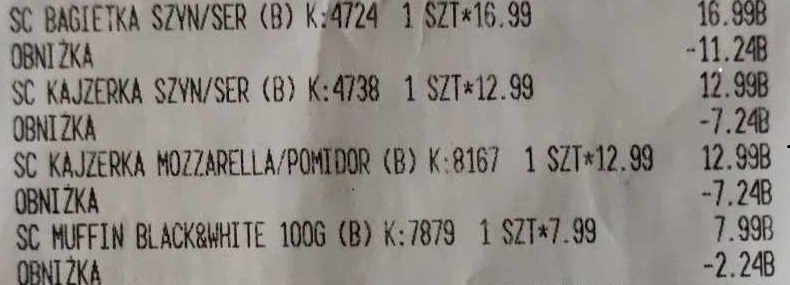
\includegraphics[width=0.6\textwidth]{images/sample_receipt.jpg}
    \caption{Sample receipt image}
    \label{fig:sample_receipt}
\end{figure}

After applying OCR (using PaddleOCR), the textual output was manually annotated with category labels and associated costs.
Below is an example of annotated receipt data in CSV format:

\begin{verbatim}
"SC BAGIETKASZYN/SER BK47241SZT*16.9S 16.99B",Food,16.99
"OBNIZKA -11.24B",Discount,11.24
"SCKAJZERKASZYN/SERBK:47381SZT*12.99 12.99B",Food,12.99
"OBNIZKA -7.248",Discount,7.24
"SC KAJZERKA MOZZARELLA/POMIDOR (B)K81671 SZT*12.99 12.99B",Food,12.99
"OBNIZKA -7.248",Discount,7.24
"SC MUFFIN BLACK&WHITE100G BK:78791SZT*7.99 7.99B",Food,7.99
"OBNIZKA -2.24B",Discount,2.24
\end{verbatim}
\noindent This structured textual data serves as input for subsequent preprocessing, embedding generation, and classification steps detailed in earlier sections.


\section{Implementation Examples}

\subsection{Text Preprocessing}

The following example shows a text normalization function used after OCR extraction to reduce noise and standardize textual data:

\begin{lstlisting}[language=Python, caption={Post-OCR text preprocessing}, label={lst:preprocessing}]
def preprocess_text(text):
    text = re.compile('[%s]' % re.escape(string.punctuation)).sub(' ', text)
    text = re.sub(r'\s+', ' ', text)
    text = re.sub(r'[^\w\s]', '', text.strip())
    text = re.sub(r'\d', ' ', text)
    text = re.sub(r'\s*\b[a-zA-Z]\b\s*', ' ', text).strip()
    return text
\end{lstlisting}
\label{code:preprocessing_example}
\noindent This preprocessing step standardizes the extracted OCR text by removing punctuation, numbers, single characters, and excessive whitespace, thus improving subsequent embedding quality.

\subsection{OCR Pipeline}

Below is an example of PaddleOCR implementation and extraction of preprocessed data from image files:

\begin{lstlisting}[language=Python, caption={OCR class}, label={lst:ocr}]
class OCR:
    def __init__(self):
        self.paddleocr = PaddleOCR(
            use_angle_cls=True, lang='pl',
            rec_algorithm='CRNN', rec_char_type='pl'
        )

    def get_preprocessed_data(self, img_path):
        ocr_data = self.perform_ocr(img_path)
        preprocessed = []
        for line in ocr_data:
            for word_info in line:
                text = preprocess_text(word_info[1][0])
                cost = preprocess_cost(word_info[1][0])
                preprocessed.append((text, cost))
        return preprocessed
\end{lstlisting}
\label{code:ocr_pipeline_example}
\noindent This OCR pipeline leverages PaddleOCR to extract textual content from images, applying preprocessing steps to ensure high-quality inputs for further analysis.

\subsection{Sentence-Transformer Fine-tuning}

The example below demonstrates how the Sentence-Transformer embedding model (\texttt{all-MiniLM-L6-v2}) was fine-tuned using contrastive loss to better capture domain-specific semantics:

\begin{lstlisting}[language=Python, caption={Fine-tuning Sentence-Transformer embeddings}, label={lst:embedding_finetuning}]
model.fit(
    train_objectives=[(train_dataloader, loss)],
    evaluator=evaluator,
    epochs=epochs,
    warmup_steps=warmup_steps,
    evaluation_steps=len(train_dataloader),
    output_path=path,
    save_best_model=True,
)
\end{lstlisting}
\label{code:finetuning_example}
\noindent Fine-tuning was performed using labeled pairs of receipt texts to ensure embeddings accurately reflect semantic differences relevant to categorization tasks.

\subsection{Hydra-driven Model Training Pipeline}

The Hydra framework was utilized for structured experimentation, enabling easy parameter adjustments and reproducibility:


\begin{lstlisting}[language=Python, caption={Training pipeline}, label={lst:preprocessing}]
@hydra.main(config_path="./conf", config_name="config")
def main(cfg):
    dataloader=Dataloader(Path(cfg.datapath))
    embedding_model=Embedding.load_mini_model(
      cfg.embeddingmodel.model_path
    )

    train_batch, test_batch, _ = Dataloader
      .get_training_ready_data(
        embedding_model, split_size=cfg.split_size
    )

    model = XGBoost(**cfg.params)
    model.fit(train_batch['embeddings'], train_batch['category'])
    results = model.test_model(
        test_batch['embeddings'], 
        test_batch['category']
    )
    hydra.utils.log.info(f'Test F1 Score: {results["f1_score"]}')
\end{lstlisting}
\label{code:hydra_pipeline_example}
\noindent Using Hydra streamlined experimentation, provided automated logging of parameters and results, and ensured experimental reproducibility.



\section{Additional Figures and Tables}
\subsection{XGBoost Hyperparameters by Model Type}

\noindent The hyperparameters used for the XGBoost classifier differ slightly depending on the embedding configuration.
Below are the tuned values for each scenario.

\begin{lstlisting}[language=yaml, caption={XGBoost hyperparameters – BERT model}, label={lst:bert_params}]
learning_rate: 0.3
max_depth: 5
n_estimators: 50
subsample: 0.8
colsample_bytree: 1.0
min_child_weight: 5
gamma: 0.1
reg_alpha: 0.0
reg_lambda: 0.0
\end{lstlisting}

\begin{lstlisting}[language=yaml, caption={XGBoost hyperparameters – Sentence-Transformer (GPT + real fine-tuned)}, label={lst:gpt_real_params}]
learning_rate: 0.2
max_depth: 7
n_estimators: 500
subsample: 0.5
colsample_bytree: 0.6
min_child_weight: 7
gamma: 0.0
reg_alpha: 0.0
reg_lambda: 0.0
\end{lstlisting}

\begin{table}[h]
  \centering
  \caption{Full classification report – BERT model (out-of-the-box, no fine-tuning)}
  \label{appendix:bert-report-outofbox}
  \begin{tabularx}{\textwidth}{lcccc}
    \toprule
    \textbf{Class} & \textbf{Precision} & \textbf{Recall} & \textbf{F1 Score} & \textbf{Support} \\
    \midrule
    Beverages (0)     & 0.25 & 0.14 & 0.18 & 7 \\
    Discount (1)      & 1.00 & 0.67 & 0.80 & 6 \\
    Food (2)          & 0.78 & 0.89 & 0.83 & 55 \\
    Healthcare (3)    & 0.50 & 0.67 & 0.57 & 6 \\
    Housing (4)       & 0.00 & 0.00 & 0.00 & 4 \\
    Other (5)         & 0.86 & 0.60 & 0.71 & 10 \\
    \midrule
    \textbf{Macro Average}   & 0.56 & 0.49 & 0.51 & 88 \\
    \textbf{Weighted Average}& 0.71 & 0.73 & 0.71 & 88 \\
    \textbf{Overall Accuracy}& \multicolumn{4}{c}{0.7273} \\
    \textbf{Overall F1 Score}& \multicolumn{4}{c}{0.7073} \\
    \bottomrule
  \end{tabularx}
\end{table}

\printbibliography

\beforelastpage

\end{document}
